\chapter{引言}
\label{cha:intro}
\section{研究背景}


随着社会发展以及人民生活水平提高,智能机器人、无人驾驶、虚拟现实等新兴技术逐渐走入人们的视野,并悄无声息的改变的人们的生活方式。而实现这些技术的核心问题之一,是如何使计算机能够理解传感器采集到的各种信号,并准确地作出响应,将决策合理反馈到真实世界。

在所有传感器信号中,视觉信号中蕴含的信息量远远大于非视觉信号,且占据了绝大部分比例。正如中国的古话所言:“一图胜千言”、“耳听为虚,眼见为实”。因此,让计算机更加准确的理解视觉信号,是不可或缺的关键任务。

计算机视觉就是一门研究如何让计算机更好完成上述任务的学科。对于人类来说,认识、理解与分析生活中常见的图像、视频等内容,是一件易如反掌、信手掂来的任务。然而对于计算机而言,完成好同样的任务却难于上青天。与人类的视角不同,在计算机中,图像、视频等信息都是以一个实值张量的形式存储的,其中每个数代表特定位置特定通道的亮度值。不像经典的排序、字符串匹配等目标很容易被形式化描述的任务,计算机视觉中的任务很难被硬编码成固定算法。图 \ref{fig:classify} 以一个经典的图像分类问题为例,说明了这类任务的困难程度。

\begin{figure}[H]
	\centering
	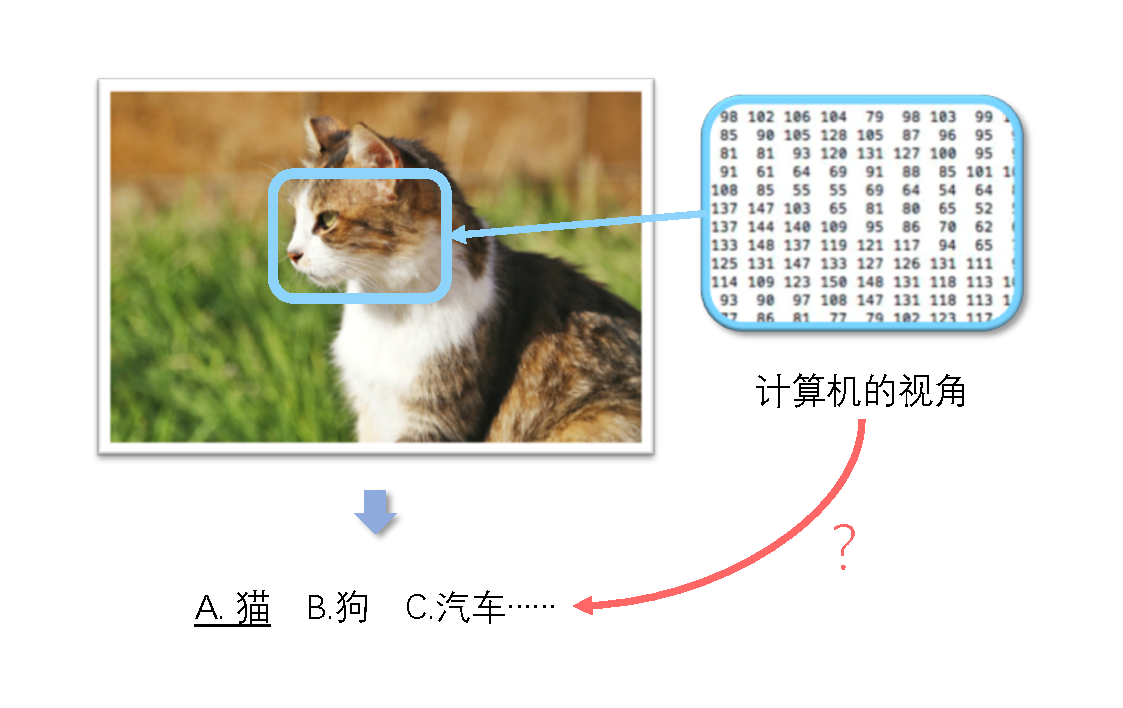
\includegraphics[width=.7\textwidth]{classify}
	\caption{图像分类问题}
	\label{fig:classify}
\end{figure}

\subsection{手工设计特征与二维深度学习}
在早期的计算机视觉研究中,人们使用了一些手工设计的方法,来提取图片和视频的局部和全局特征,并将其作为输入的一种特殊表示。比较经典的特征提取方法有
Gabor 变换\cite{gabor}、Canny 边缘检测\cite{canny}、Harris角点检测\cite{harris}、
尺度不变特征变换 (Scale-invariant Feature Transform, SIFT)\cite{sift}、
方向梯度直方图 (Histogram of Oriented Gradient, HoG)\cite{hog, hog2}、词袋模型 (Bag-of-words Model, BoW Model) \cite{bow} 等。这些经典算法得到的特征尽可能的保留了与正确结果相关的信息,同时过滤了与之无关的信息,是更加接近于输出的表示形式。
直到深度学习发展得如火如荼的今天,它们仍然在一些特定领域中被广泛应用,例如机器人的同步定位与地图构建 (Simultaneous Localization and Mapping, SLAM)\cite{slam}任务等。

然而对于不同的任务来说,我们需要的提取的信息往往是不同的。上述通用方法提取到的特征通常与具体问题无关,没有充分挖掘问题与输入数据的规律与特点。深度学习就是解决此不足的方法之一,也是近年来的研究热点。它首先将输入转化成一些简单的特征,然后再进一步将其转化为一系列相对复杂的特征,由浅入深、循序渐进地将输入一步步变换为正确输出。与早期研究不同,这些特征是通过机器自动学习得到的,而非手工设计得到的。

因为需要通过机器从已有的训练数据中自动学习到特征,所以深度学习算法是一种数据驱动的算法,而且其成败与数据的优劣密不可分。随着社会数字化的推广与互联网技术的普及,海量的互联网数据变得容易收集与管理,深度学习数据集的准备任务也不再高不可攀。近年来,我们也看到了不少优秀的大规模数据集,如 ImageNet\cite{imagenet}、Microsoft Common Objects in Context (COCO) \cite{coco}等,它们的出现极大地推动了深度学习的发展进程。



\begin{figure}[H]
	\centering
	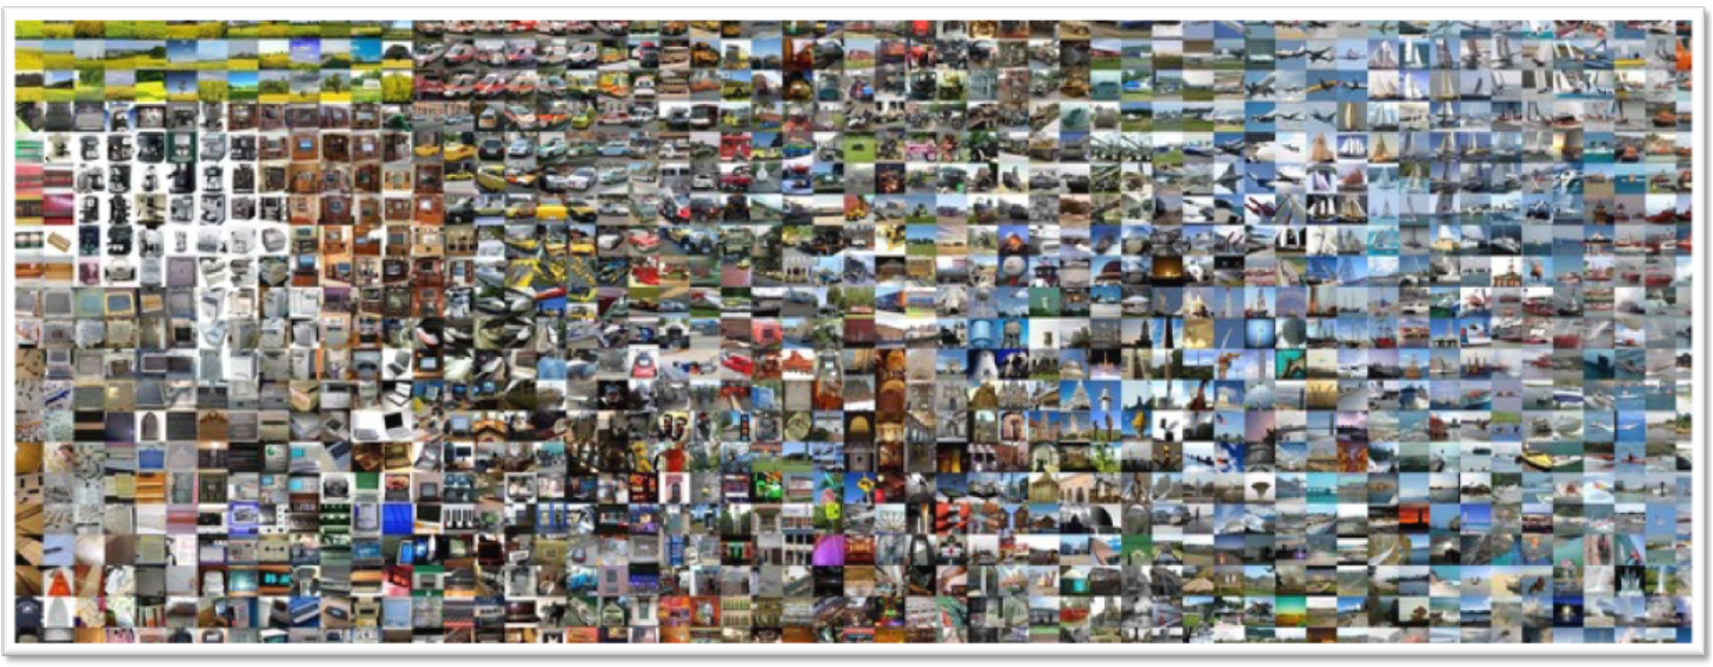
\includegraphics[width=.95\textwidth]{imagenet}
	\caption{ImageNet 数据集 \cite{imagenet}}
\end{figure}

模型的结构也是制约深度学习成败的关键因素。为了进一步提升深度学习算法的准确率,相当多的优秀工作涌现了出来,例如 AlexNet\cite{alexnet}, VGG\cite{vgg}, GoogLeNet\cite{googlenet}, ResNet\cite{resnet} 等。这些工作提出的模型在最大的对象识别比赛——ImageNet 大型视觉识别挑战 (ImageNet Large Scale Visual Recognition Competition, ILSVRC) 上一次又一次的刷新着记录,向我们展示着深度学习的强大威力。此外,不仅仅是图像分类,这些模型的思想还被用于解决物体检测\cite{rcnn, fastrcnn, fasterrcnn, ssd, yolo}、图像分割\cite{maskrcnn, fcn}、图像生成
\cite{gan, dcgan, wgan, wgangp, lsgan, began, pggan, sngan, cvaegan}等其他问题,并取得了相当可观的结果。

\begin{figure}[h]
	\centering%
	\subcaptionbox{物体检测与图像分割\cite{maskrcnn}}
	{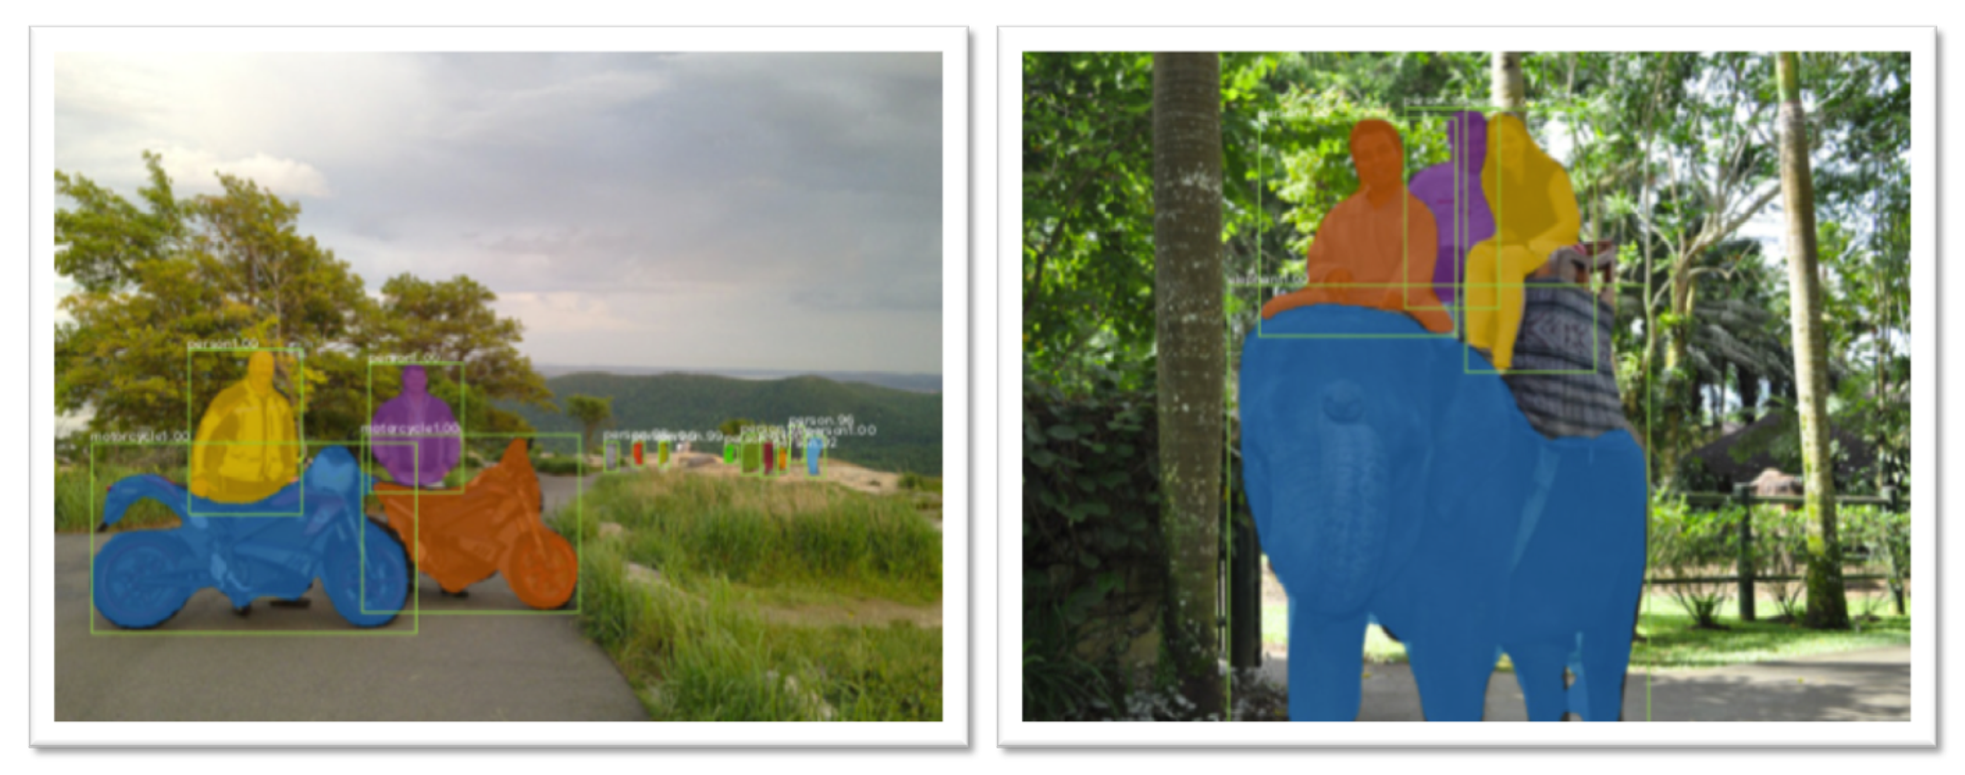
\includegraphics[width=.45\textwidth]{maskrcnn}}%
	\hspace{2em}%
	\subcaptionbox{图像生成\cite{cvaegan}\label{fig:2dgen}}
	{\includegraphics[width=.45\textwidth]{CVAE-GAN}}
	\caption{深度学习在众多问题上都取得了突破性的进展}
\end{figure}

\subsection{三维深度学习}

尽管计算机视觉在深度学习的帮助下取得了里程碑式的成果,遗憾的是它们却基本上服务于平面图像与视频等二维数据。

众所周知,
我们生活在一个三维的世界,每天都不可避免地需要与三维模型接触。而在机器人定位、虚拟现实、医学图像处理等特定任务中,
三维数据%相比于传统的二位数据,
更是占据了举足轻重的地位。因此,让计算机学会认识、理解与分析三维物体,同样是计算机视觉中的重要课题之一。我们将使用深度学习解决上述问题的方法统称为三维深度学习,以示与上节中二维深度学习的区别。

对于三维深度学习的研究,我们目前才刚刚起步。
%笔者认为,
我们认为,
阻碍三维深度学习发展的因素有三点。




首先,早期研究的三维数据规模远不如二维数据。众所周知,三维数据通常由传感器采集或者由艺术师设计。由于人力物力等客观因素的限制,能够被收集到的三维数据屈指可数。
% 深度学习等数据驱动算法的表现也必将受限于数据的规模。
这也成为了深度学习等数据驱动算法的主要瓶颈之一。

在互联网还没有普及的时代,人们曾通过三维扫描仪器和数学建模等方法,制作了 Stanford Bunny 兔子和 Utah 茶壶等经典模型。如同程序设计教程中的 \texttt{"Hello World"} 例程一样,如今它们也成为了计算机图形学中标准测试模型。
对于计算机图形学的渲染任务来说,因为其重点研究对象,如渲染方程\cite{renderequ}与双向反射分布函数 (Bidirectional Reflectance Distribution Function, BRDF)\cite{phong, blinnphong} 等,对需要被渲染的模型没有任何假设,具有一般性和通用性,因此少量标准模型的提出已经足够学科自身的发展。相反的,三维深度学习中的大部分问题却高度依赖于待处理三维模型的统计信息和分布规律,而这不可能从两个模型中直接得到。因此,它们并不能对三维深度学习带来实质性的帮助。
% 更不可能将它们作为深度学习算法的训练数据集,以训练出有效的模型解决实际的问题。


\begin{figure}[h]
	\centering%
	\subcaptionbox{Stanford Bunny 兔子}
	{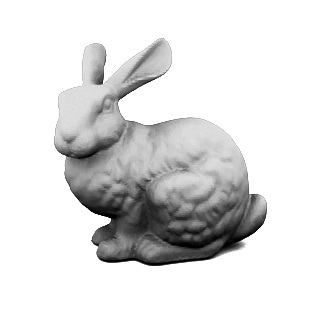
\includegraphics[width=.3\textwidth]{bunny}}%
	\hspace{2em}%
	\subcaptionbox{Utah 茶壶}
	{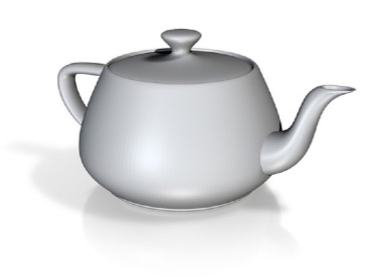
\includegraphics[width=.3\textwidth]{utah}}
	\caption{人们在早期使用的三维模型}
\end{figure}


“巧妇难为无米炊”,缺少必要训练数据,再强大的深度学习算法也无用武之地。随着互联网的普及,Princeton Shape Benchmark 数据集\cite{princetonShapeBenchmark}应运而生,极大的丰富了科研人员可用的模型数据。此数据集 包括了约 \numprint{1814} 个三维模型,分为 92 个大类。与 Stanford Bunny 兔子和 Utah 茶壶相比,虽然它在数据规模上确实有了一定的提升,但这对于深度学习所需的庞大数据量而言只是杯水车薪。它不足以让深度学习算法从中充分地挖掘出三维模型的内在规律,也不能让深度学习在相关任务中充分发挥其强大潜力。

\begin{figure}[H]
	\centering
	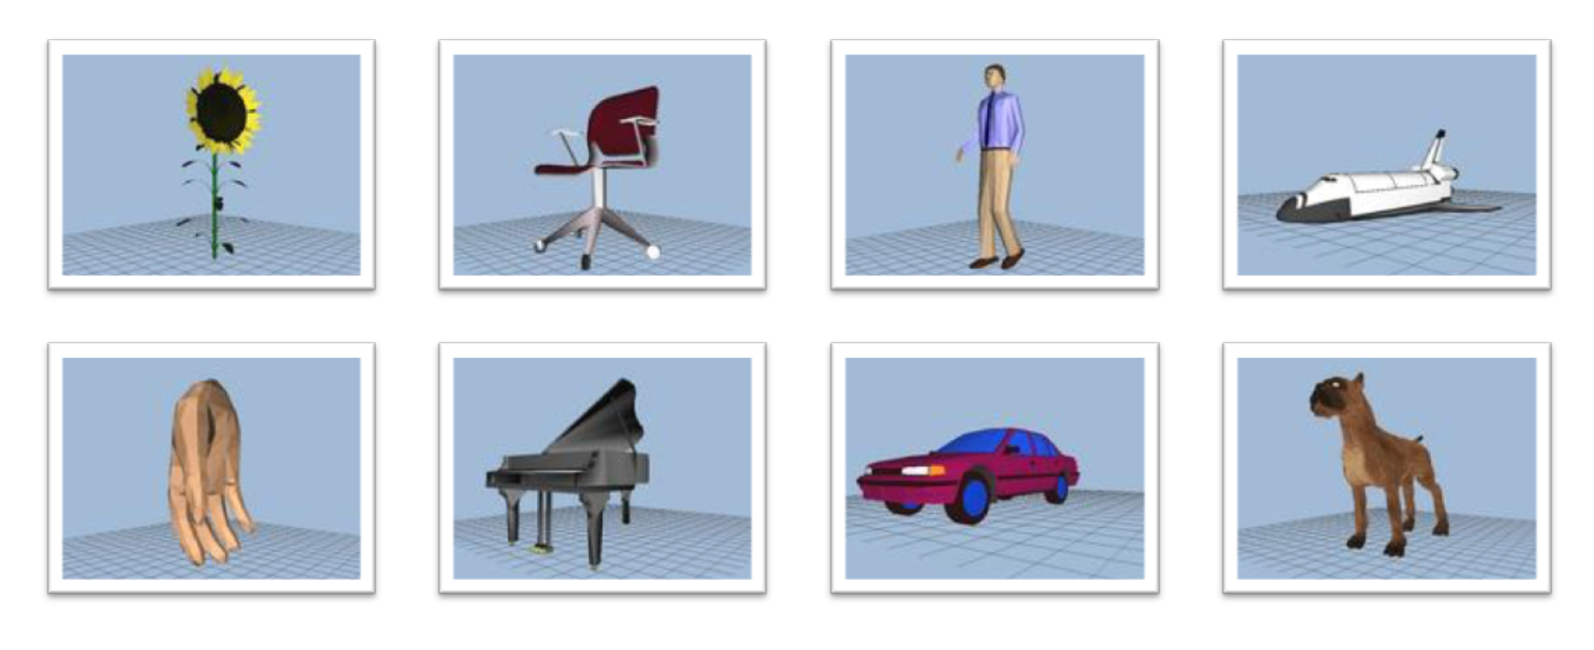
\includegraphics[width=.83\textwidth]{princeton}
	\caption{Princeton Shape Benchmark 数据集\cite{princetonShapeBenchmark}}
\end{figure}

随着计算机辅助设计 (Computer Aided Design, CAD) 系统的增强以及三维扫描设备的进一步发展,
近年来能在网络上收集到的三维模型规模有了可观的提升。
众多的三维模型仓库也不断地在互联网平台上涌现,如 Google Sketchup, 3D Houseware, Clara.io, Sketchfab 等。这些仓库均能提供至少数以万计的三维模型,让三维深度学习不再因为训练数据的短缺而止步不前。后来,人们对这些数据进行了进一步的整理和预处理,提出了 ShapeNet 数据集\cite{shapenet}。它与早期的数据集相比,规模更大,内容更丰富,共包含了 \numprint{51300} 个模型,分为 \numprint{55} 个大类。这很大程度地简化了三维深度学习的数据收集工作,为三维深度学习的发展做好了铺垫与准备。


\begin{figure}[H]
	\centering
	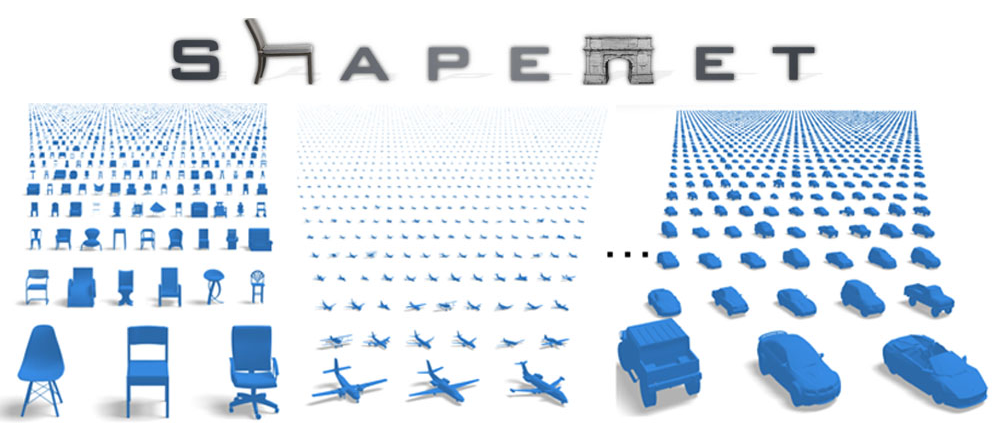
\includegraphics[width=.95\textwidth]{shapenet}
	\caption{ShapeNet 数据集\cite{shapenet}}
\end{figure}



% 另一个制约三维深度学习的因素是模型的表示方式
数据集规模并不是三维深度学习的唯一瓶颈,事实上,三维模型的表示方式同样制约着三维深度学习的发展。目前,三维模型的表示方式没有统一的规范。实际上,不同的表示方式也没有优劣之分,它们都可以在特定的需求和应用场景下发挥着无法替代的作用。
例如,将生成的三维模型通过光线追踪算法进行渲染时,我们通常需要提供模型的三角面片而非点云,因为后者不能提供法向等关键信息;而分析三维扫描设备获取的模型信息时,我们通常使用点云而非三角面片,因为后者并不是传感器采集到的原始数据。

三维模型表示的多样性也使得三维深度学习分化为了许多不同的流派。目前,三维深度学习中常见的表示方式有五种:多视角图像\cite{mvcnn1, mvcnn2, mvcnn3}、体素\cite{3dcnn, fpnn, octnet, ocnn, 3dr2n2, octgen}、三角面片\cite{surfnet, surfacecnn, syncspeccnn}、点云\cite{pointnet, pointnet2, kdnet, pointcnn, pointsetgen}以及基于 CAD 原语的参数化表示\cite{volumetricprimitives, grass}
%,如图 \ref{fig:rep} 所示
。其中,前两者是规则型的表示,所有数据都以张量的形式有规则地排列,就像图片和视频一样,故二维深度学习中的思想和算法能够直接应用于这类形式的数据;后三者是非规则型的表示,不能与已知的数据形式类比,也没有二维深度学习的算法能直接处理。目前,非规则型的表示成为了当今三维深度学习的重点研究方向。

\begin{figure}[h]
	\centering%
	\subcaptionbox{多视角图像\cite{mvcnn1}}
	{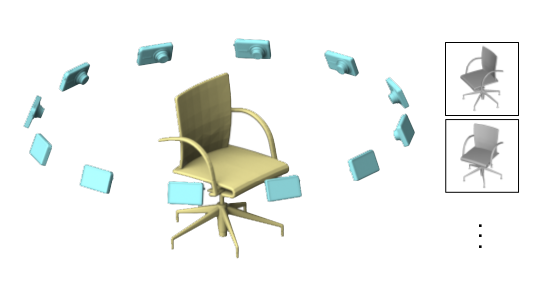
\includegraphics[height=3.4cm]{mv}}%
	\hspace{1em}%
	\subcaptionbox{体素\cite{octgen}}
	{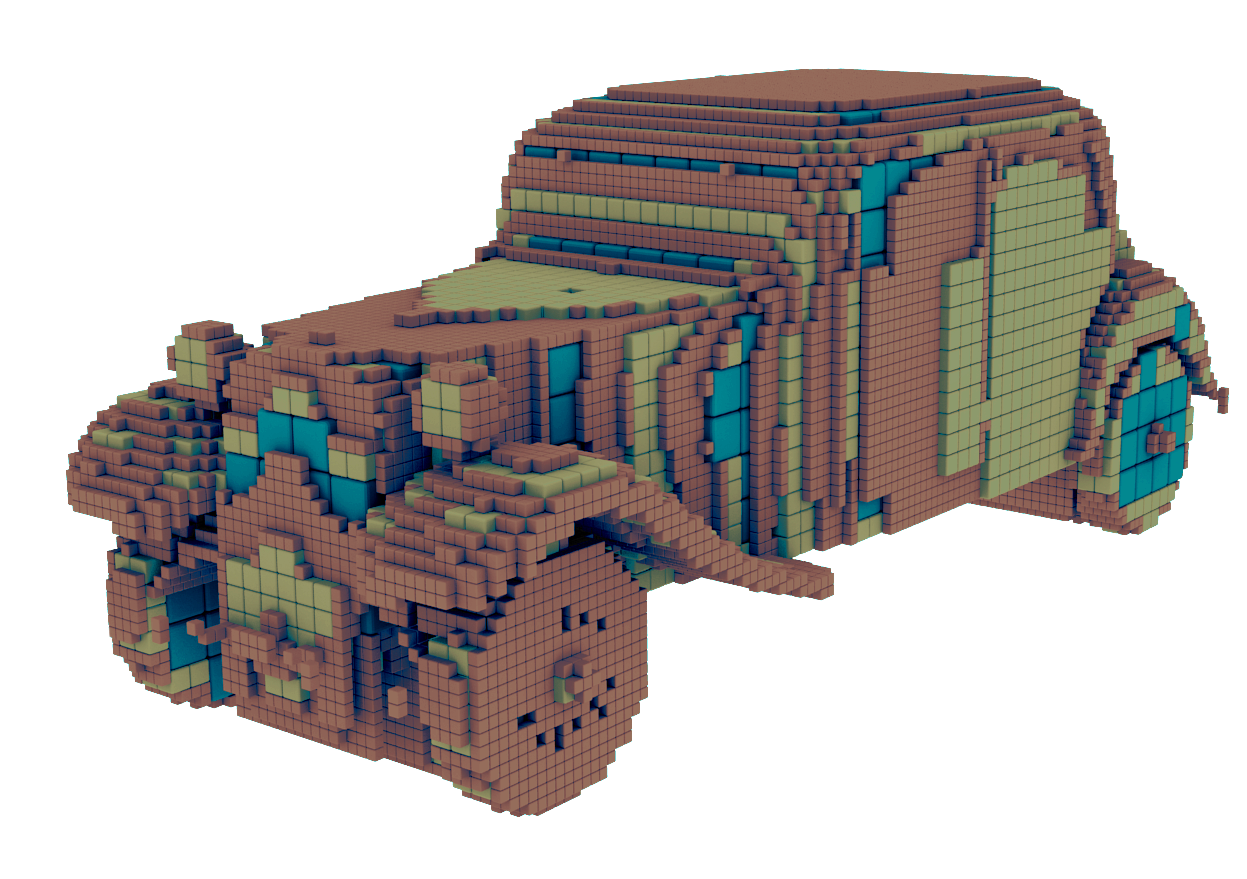
\includegraphics[height=3.4cm]{vox}}%
	\\
	\vskip1.5em
	\subcaptionbox{三角面片\cite{syncspeccnn}}
	{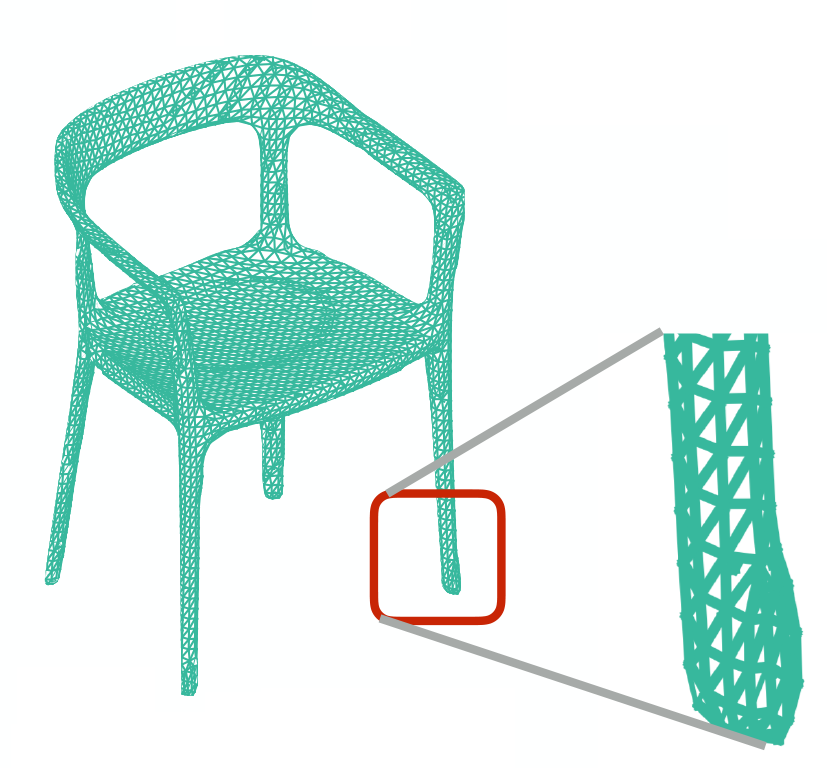
\includegraphics[height=3.4cm]{pm}}%
	\hspace{1em}
	\subcaptionbox{点云\cite{pointsetgen}}
	{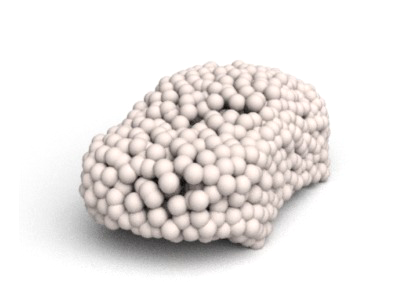
\includegraphics[height=3.4cm]{pc}}%
	\hspace{1em}
	\subcaptionbox{CAD 原语\cite{grass}}
	{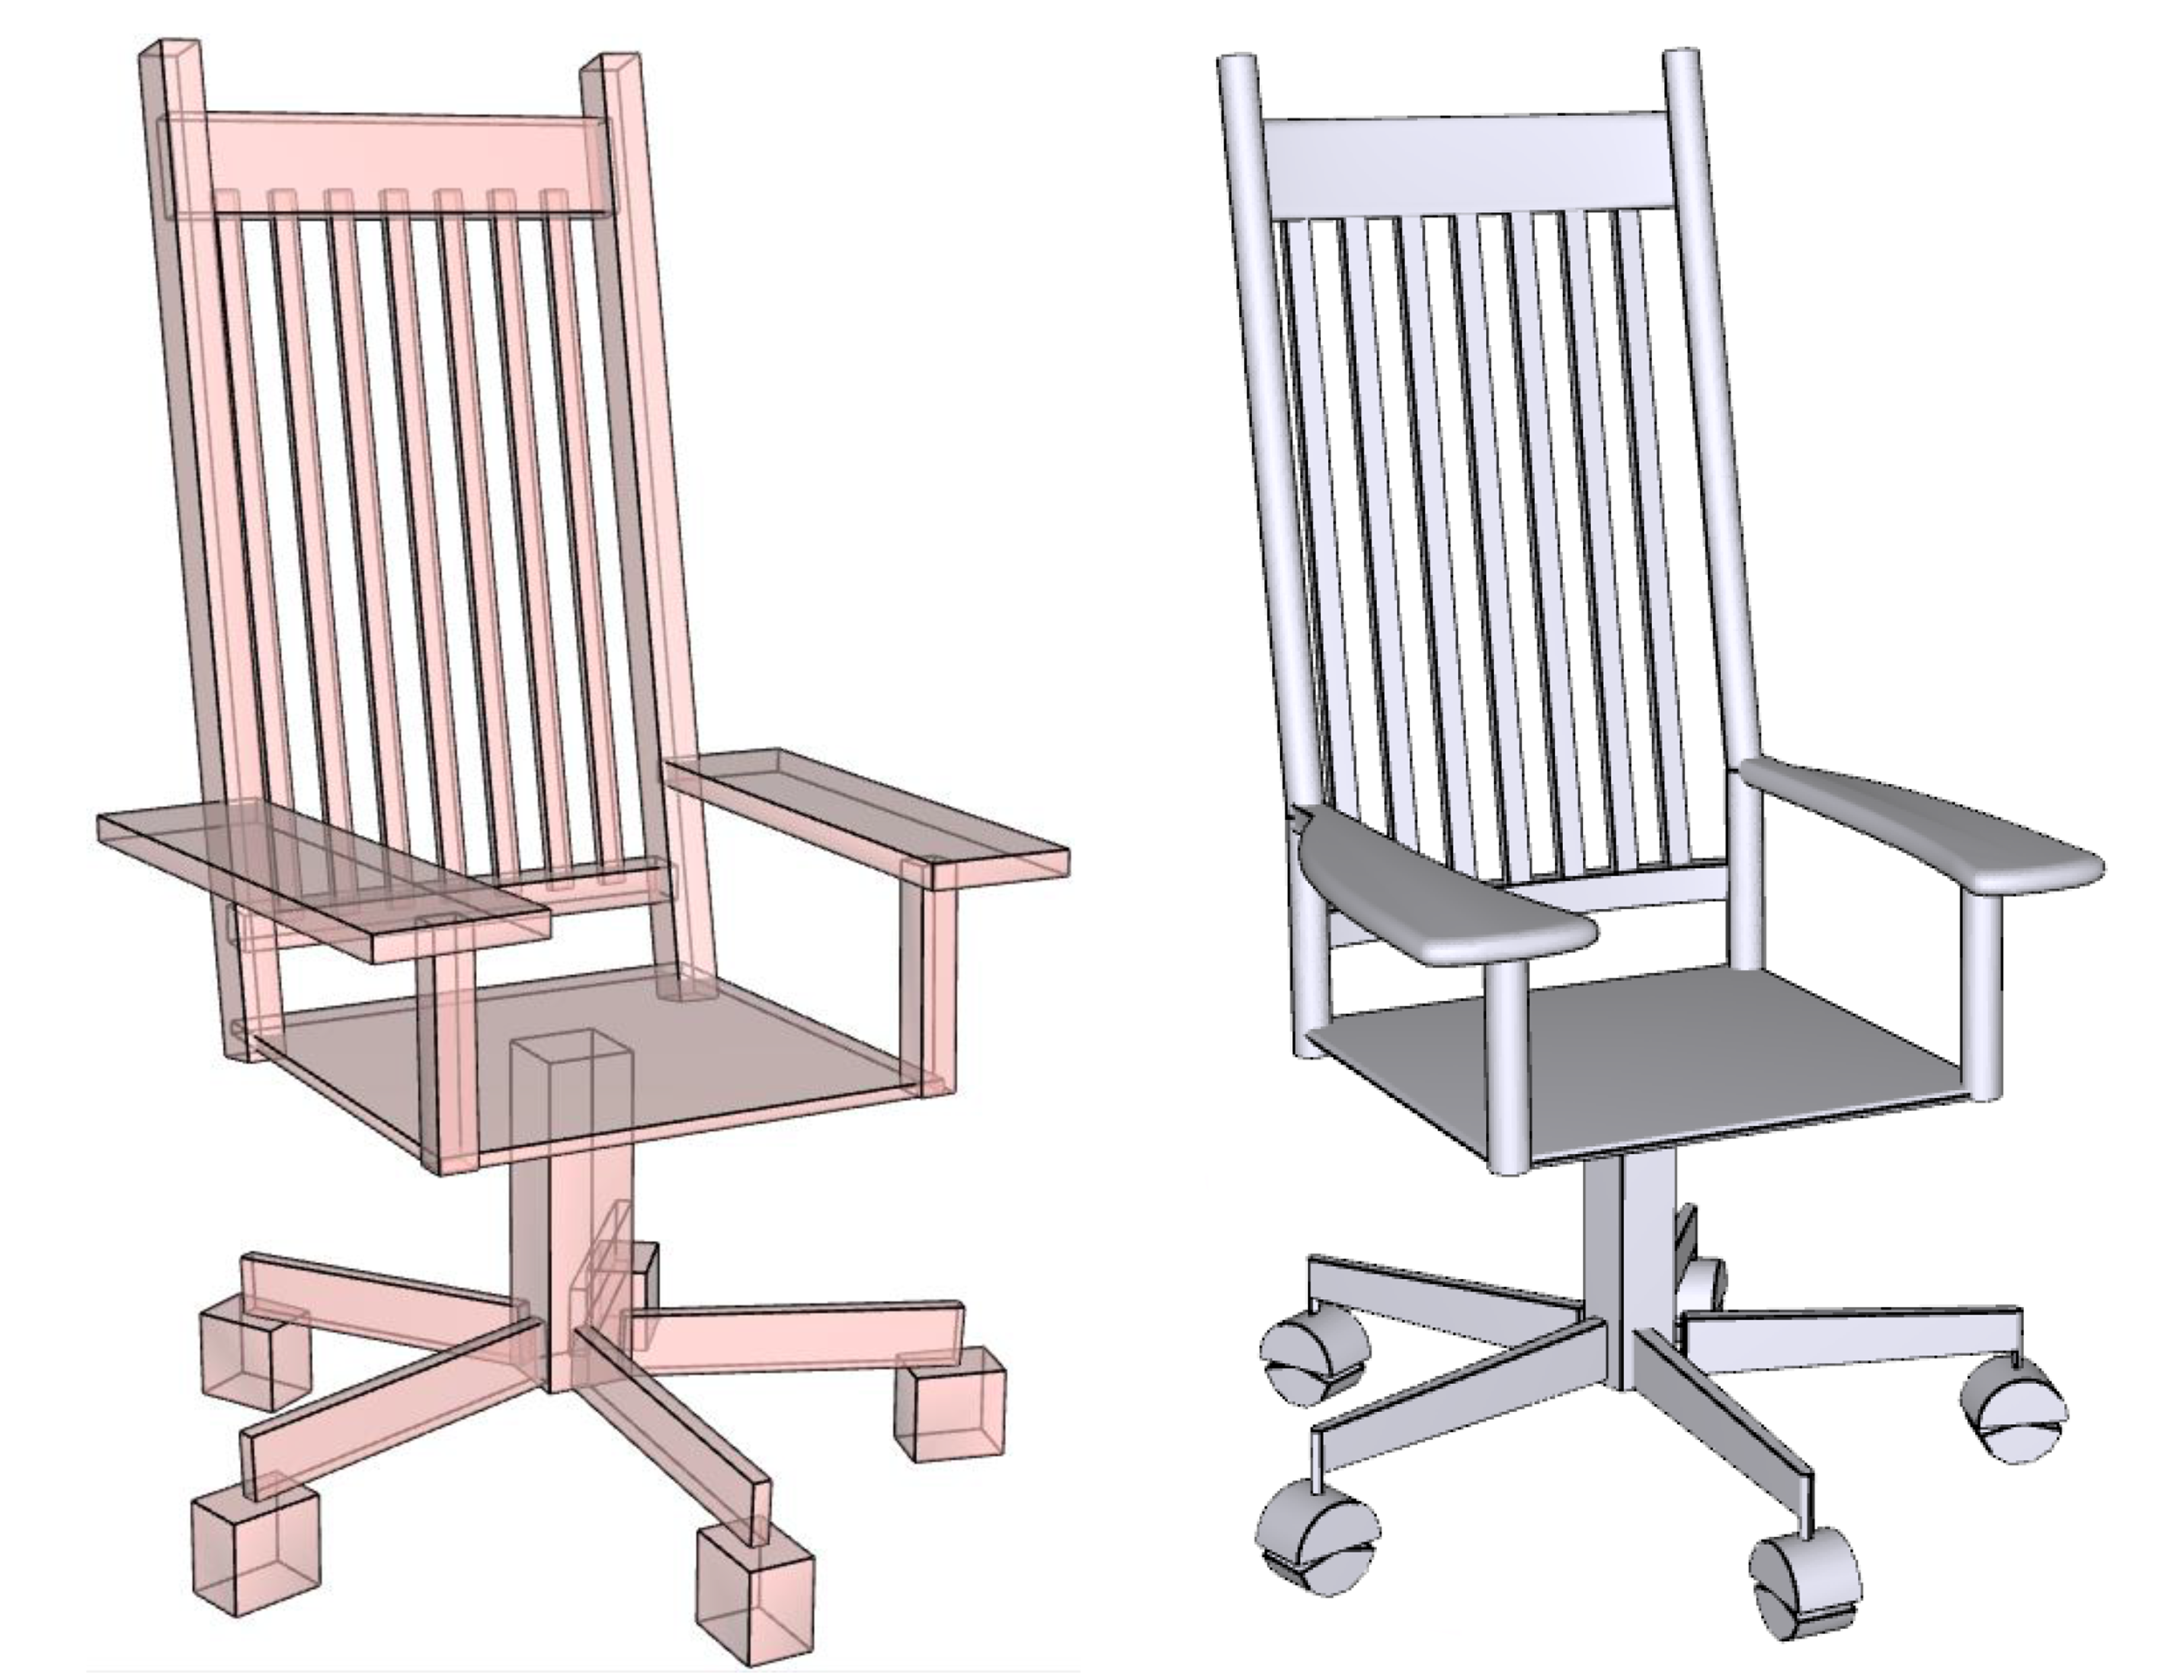
\includegraphics[height=3.4cm]{cad}}
	\caption{三维深度学习中常见的五种表示方式}
	\label{fig:rep}
\end{figure}


最后一个制约三维深度学习的因素是三维数据自身的大小。在表现形式上,三维数据比图像等二维数据多了一维,因此要直接借用二维深度学习的思路达到与之等效的结果,计算量至少需要增长一个数量级。这通常是客观条件所不允许的。

以体素表示为为例,经典的 AlexNet\cite{alexnet} 使用了尺寸为 $224 \times 224$ 的 RGB 图像作为输入,如果把它直接扩展为 $224 \times 224 \times 224$ 三维体素表示,则硬件需求和计算时间至少要增加两百倍。在时间和硬件资源的双重限制下,我们不得不作出折衷和妥协。例如, 3DShapeNets\cite{3dcnn} 使用了一个 $30 \times 30 \times 30$ 的三维体素表示作为输入,这虽然与 AlexNet 的计算量在数量级上基本持平($224^2 = \numprint{50176} \approx \numprint{27000} = 30^3$),但低分辨率的采样操作使得三维模型的质量大打折扣。

值得庆幸的是,并不是所有的表示方式都像体素一样庞大。
点云就是这样一种简约的表示方式,其本质是在三维模型的二维表面上进行采样,形式上记录着三维的信息,但实则只有二维的数据量。虽然没有经典的二维深度学习方法可以直接借鉴,但只要设计好合理的方式进行处理,点云这种新兴的表示方式必将为三维深度学习指出一条崭新的出路。

本文的研究正是从点云表示出发,探索其能在多大程度上改善三维深度学习的表现。

%\begin{figure}[h]
%  \centering%
%  \subcaptionbox{三角面片表示}
%    {\includegraphics[width=.4\textwidth]{utah-mesh}}%
%  \hspace{3em}%
%  \subcaptionbox{体素表示}
%    {\includegraphics[width=.4\textwidth]{utah-vox}}
%  \caption{低分辨率体素化表示}
%\end{figure}

%此外,这样的妥协还会


\section{研究现状}

三维深度学习中研究的问题是二维深度学习的继承和拓展,其外延不仅包括二维深度学习中的常见问题,如分类\cite{pointnet}、检测\cite{frustumpointnet}、分割\cite{pointnet}、生成\cite{latentpc}等,还包括一些三维深度学习中独有的问题,如视角恢复\cite{rendercnn},三维重建\cite{pointsetgen},形状补全\cite{shapecomplete}等。在实际应用中,无论被处理的三维模型是以何种表达形式呈现的,求解这些问题的需求是客观存在的。
因此,各种流派的三维深度学习可以按照问题目标被进一步细分。

目前,点云相关的三维深度学习研究进展得如火如荼。针对点云的各种处理需求,人们提出了多种不同的模型与算法来灵活应对和处理。限于篇幅,此处列举并简要介绍与本文相关性最大的三个工作。各工作的具体细节,我们将在第 \ref{cha:3d_deep_learning}、\ref{cha:gen}  章中予以详细说明。

\subsection{基于图片的三维点云重建}

PointSetGen\cite{pointsetgen} 是第一个将点云引入三维深度学习的工作,开创了历史先河。此工作的核心目标是希望从输入的单张 RGBA 图像中直接重建出物体的三维结构,并以点云的形式输出结果,如图 \ref{fig:pointsetgen} 所示。


\begin{figure}[h]
	\centering%
	{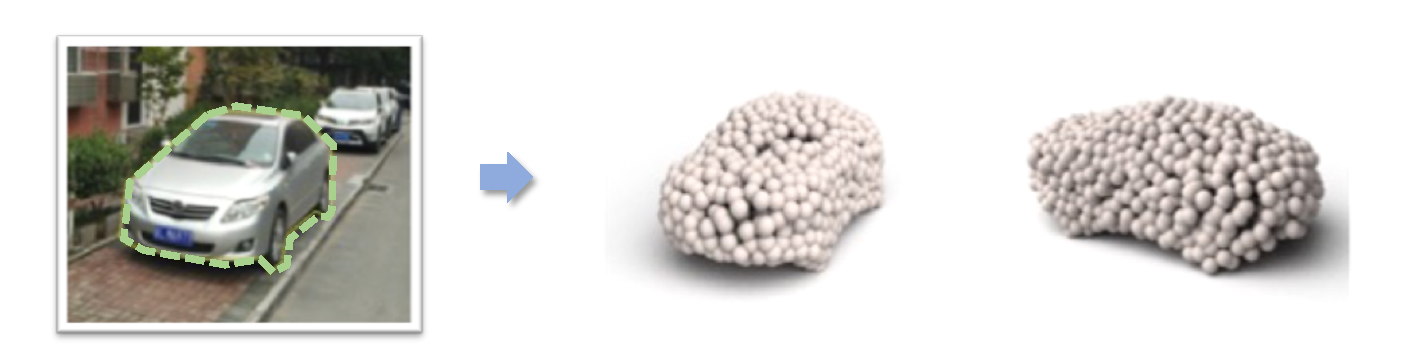
\includegraphics[width=.95\textwidth]{pointsetgen}}
	\caption{基于图片的三维点云重建:PointSetGen\cite{pointsetgen}}
	\label{fig:pointsetgen}
\end{figure}

此工作最大的贡献在于提出了点集 $S = \{(\bm p_i)\}_{i=0}^{N - 1}$ 之间的度量方案——Chamfer 距离 (Chamfer Distance, CD) 和 推土机距离 (Earth Mover's Distance, EMD):
\begin{align}
	\DCD{S_1}{S_2}  & =
	\sum_{\bm p \in S_1} 􏰘\min_{\bm q \in S_2} \Norm*{\bm p - \bm q}^2 +
	\sum_{\bm q \in S_2} 􏰘\min_{\bm p \in S_1} \Norm*{\bm p - \bm q}^2 \label{eq:cd} \\
	\DEMD{S_1}{S_2} & =
	\min_{\text{双射} \phi:\, S_1 \to S_2} \sum_{\bm p \in S_1} \Norm*{\bm p - \phi(\bm p)}_2
	\label{eq:emd}
\end{align}
利用这两个度量,我们很容易定义模型输出与真实情况的差距,即损失函数。
只要
%通过
最小化上述损失函数,我们就可以得到高质量的模型,从而解决问题。

\subsection{点云数据的分类与分割}
PointNet \cite{pointnet} %的提出
主要
解决了点云数据的分类与分割问题,如图 \ref{fig:pointnet} 所示。

\begin{figure}[h]
	\centering%
	{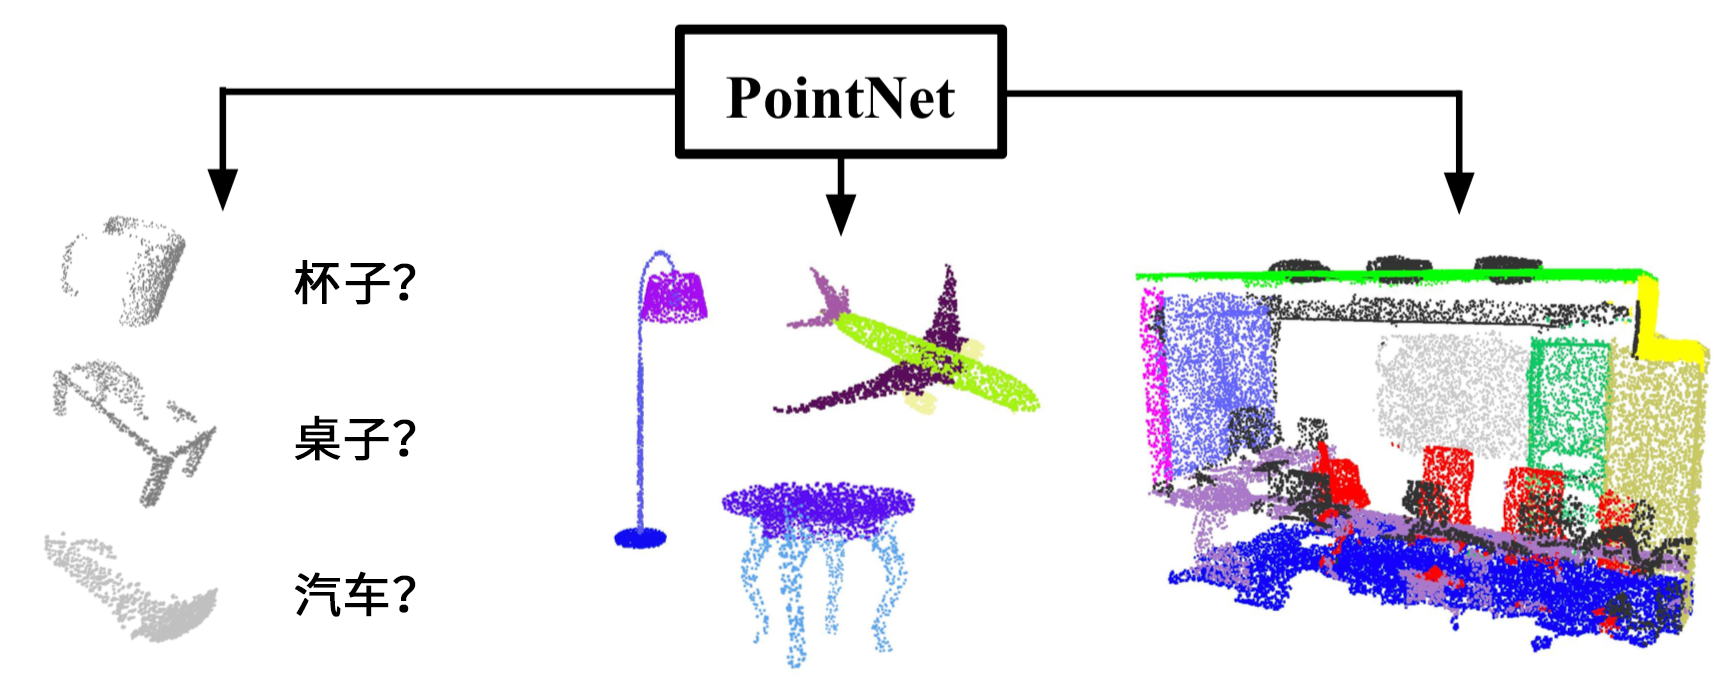
\includegraphics[width=.95\textwidth]{pointnet}}
	\caption{点云数据的分类与分割:PointNet \cite{pointnet}}
	\label{fig:pointnet}
\end{figure}

此工作从点集的排列不变性入手,提出了使用对称函数来处理点云输入的观点。

对称函数是一类数学函数,其输出不随输入变量的排列而发生变化。例如对一组数相加、相乘、求最大值或者最小值等,都是对称函数。%而
点云的分类和分割同样是对称函数。
容易观察到,如果存在映射 $h: \mathbb{R}^3 \to \mathbb{R}^K,
	g: \underbrace{\mathbb{R}^K \times \mathbb{R}^K \times \cdots \times \mathbb{R}^K}_{N} \to \mathbb{R}^K, \gamma: \mathbb{R}^K \to \mathbb{R}$,且 $g$ 为对称函数,则映射 %$f: S \to \mathbb{R}$
\begin{align}
	f(\{\bm p_1, \ldots, \bm p_N \}) = \gamma \circ g(h(\bm p_1), \ldots, h(\bm p_N)) \label{eq:symmetric}
\end{align}
亦为对称函数。
只要把 \eqref{eq:symmetric} 作为模型架构,并
取 $g$ 为 多个向量的逐元素最大值 (Element-wise Maximum) % $g = \max$ 
等简单的对称函数,$h, \gamma$ 为一个深度神经网络,就可以近似出一个合理的模型以解决问题。


\subsection{点云数据的隐表示与自动生成模型}
近年来,深度学习的研究热点逐渐从分类问题转向了生成问题。目前最前沿的图像生成结果已经达到了以假乱真的地步,而且还在不断的提升,如图 \ref{fig:2dgen} 所示。
那么,点云生成能否做到这样的程度呢?

文献 \inlinecite{latentpc} 的工作对此做出了肯定的回答。
通过将已有的点云深度学习算法与深度生成算法相结合,我们可以生成出多样的三维模型,且达到了与图像生成相似的结果。

值得注意的是,这个算法并不是直接在已有数据集中随机抽取一个输出,而是实实在在的学习到了三维模型内在的统计规律,
并依此举一反三地生成全新的三维模型。这样的算法可以对输出结果做插值和代数操作,是
%前者
朴素算法
所不能比拟的。


% PointGAN 


\section{本文的主要工作与贡献}


% 本文的工作是对基于点云的三维深度学习的一次摸索与尝试。


%我们
本文要解决的核心任务是进一步提升点云三维重建的质量。
具体地,我们首先使用已有算法,实现了一套基于单物体单图像的三维点云重建系统。
其读取单张 RGB 图像,自动生成 mask,并以点云的形式重建并输出图中物体的三维形态。
随后,我们将已有的重建算法与图像生成任务中的经典算法进行了有机的结合,不仅提高了原算法的重建质量,而且还增强了输出的多样性,使得算法的输出结果更加真实,同时能生成出更多的模型,而不受限于仅有的输入图像。

例如,用户可以对于多张不同图片的重建结果进行加权平均,生成出介于各个模型间的一个中间形态。这在用户不容易得到目标物体图像的情况下很有意义。
值得注意的是,这并不是通过直接对输出结果进行插值实现的,而是对于隐表示进行操作的结果,因为前者这样的素朴处理方式和并不一定能生成合理的结果。

综上所述,本文的主要贡献有:
% \begin{itemize}
%   \item 提出了一套更加自动、用户友好的三维重建系统:用户不必像已有算法一样花费大量时间提供 mask 信息;
%   \item 改善了已有工作的重建质量:已有算法重建失败时,本文算法仍然能给出合理的重建结果;
%   \item 增加了模型的生成能力:%本文提出的算法
%   本工作能生成的物体并不局限于输入图像中记录的对象。
% \end{itemize}
% 本文的主要贡献有:
\begin{itemize}
	\item 提出了一套更加自动、用户友好的三维重建系统:通过整合已有技术,用户不必再花费时间提供 mask 信息;
	      % \item 提出了一套更加自动、用户友好的三维重建系统:用户不必像已有算法一样花费大量时间提供 mask 信息;
	\item 改善了已有工作的重建质量:已有算法重建失败时,本文算法仍然能给出合理的重建结果;
	\item 增加了模型的生成能力:%本文提出的算法
	      %本工作能生成的物体并不局限于输入图像中记录的对象。
	      本文算法比已有算法更灵活,可能对多个重建结果进行插值,输出结果也更丰富多样。
\end{itemize}

\section{本文的行文结构}
本文的行文结构如下:
\begin{itemize}
	\item %在
	      第 \ref{cha:intro} 章%中,我们将
	      主要介绍了与本文工作相关的历史背景和研究现状,并说明了本文工作的主要内容与贡献;
	      % 具体的,我们计算机视觉的历史由来引入,逐步介绍了计算机视觉的研究是如何从手工设计特征出发,逐步拓展到二维深度学习与三维深度学习的。随后,我们讲解了三维深度学习的难点与分类,强调了点云三维深度学习的重要意义,并以三个点云深度学习为例进行了简要介绍。最后,我们说明了本文工作的主要内容与贡献。

	\item 第 \ref{cha:3d_deep_learning}、\ref{cha:gen} 章主要介绍了已有的工作成果,是第 \ref{cha:exp}、\ref{cha:result} 章的本文工作预备与铺垫。其中:
	      \begin{itemize}
		      \item %在
		            第 \ref{cha:3d_deep_learning} 章
		            % 中,我们
		            详细讲解了点云三维深度学习及其重要工作 PointSetGen\cite{pointsetgen} 和 PointNet\cite{pointnet}。而前者 PointSetGen 则是本文主要参考以及改进的对象;
		      \item %在
		            第 \ref{cha:gen} 章%中,我们主要介绍
		            主要引入了深度生成模型,是本文工作的理论支撑;
		            % \item %在
		            % 第 \ref{c h a: g e n 3 d} 章%中,我们
		            % 主要讨论了基于点云的三维深度生成模型,证实了本文工作在实践上可行性;
	      \end{itemize}
	\item %在
	      第 \ref{cha:exp}、\ref{cha:result} 章%中,我们主要介绍
	      详细讲解并记录了本文工作的算法流程与实验结果,是全文的核心与关键;
	\item %在
	      第 \ref{cha:summ} 章%中,我们对
	      %是
	      简洁明晰地分析并总结了本文工作,指出了其意义与贡献,
	      %本文工作
	      %进行
	      %的
	      %分析与总结,
	      同时也
	      %并简要指出了
	      给出了未来可能的改进方向。

\end{itemize}








% 
% 
% 随着以及计算机硬件系统的发展,
% 计算机视觉已经取得了突飞猛进的进展。借助海量数据以及深度学习的方法,我们已经可以在图像分类、物体识别、
% 物体分割、图像生成等任务上取得相当可观的结果。
% 
% 
% 然而,对于三维物体的相关理解任务,我们才刚刚起步。首先,三维数据在表现形式上比图像等二维数据多了一维。
% 直接使用已有算法会使得计算量增长一个数量级,结果自然会受限于时间和硬件资源的限制。
% 其次,三维数据的表示形式多样。诸如点云、三角面片等不规则的表示,根本无法被已有算法直接处理。
% 最后,

